\documentclass[12pt, letterpaper]{article}
\usepackage[utf8]{inputenc}
\usepackage{graphicx}
\graphicspath{ {images/} }

\title{Rocks and Minerals: Everyday Uses}
\author{Francisco Javier Guijarro \thanks{funded by IES JC1}}
\date{October 2021}

\begin{document}
\maketitle
We use things made from rocks and minerals every day. The items in this case are just a few of the ways that we use rocks and minerals in our everyday lives.

\section{Gypsum, chalk and slate}

	\begin{itemize}
		\item \textbf{Gypsum} is the basis for \textbf{drywall}.
		\item \textbf{Chalkboards} are made from \textbf{slate}.
		\item \textbf{Chalk} is a limestone made of the skeletons of millions of microbes.
	\end{itemize}
	
	\begin{figure}[h]
		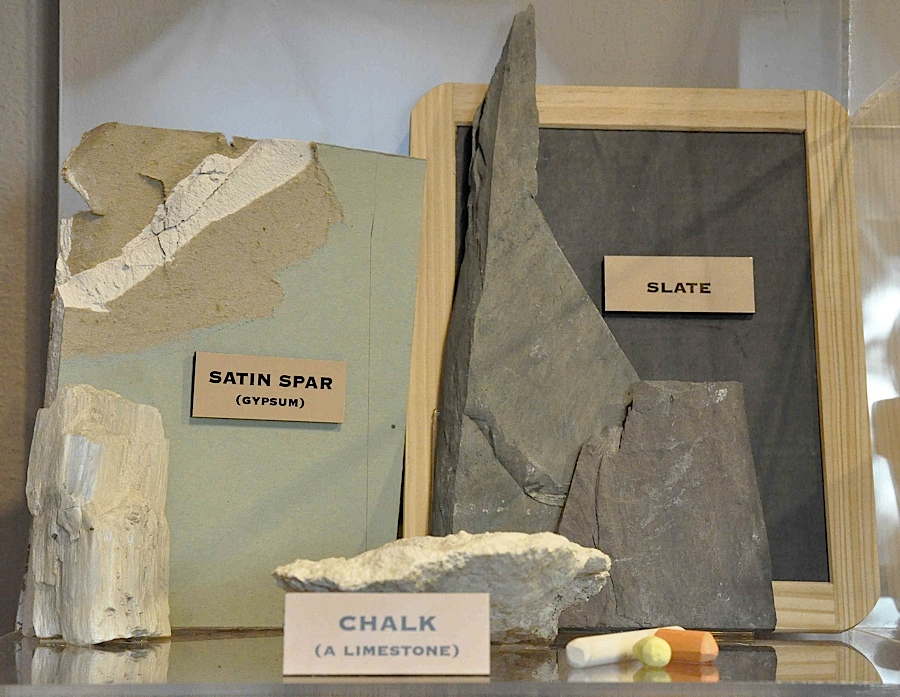
\includegraphics{shelf01}
		\centering
	\end{figure}
	
\section{Clay Mudstone}

	\par \textbf{Ceramics} are made from clay mudstone.
	
	\begin{figure}[h]
		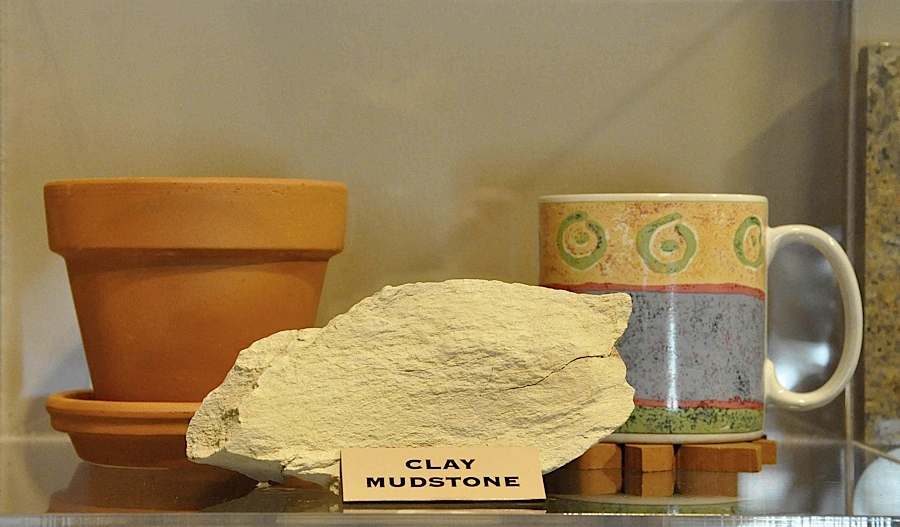
\includegraphics{shelf02_0}
		\centering
	\end{figure}

\section{Granite, Salt, Quartz and Marble}

	\begin{itemize}
		\item \textbf{Granite} and \textbf{marble} counter tops are made from stone.
		\item \textbf{Salt} is and essential nutrient.
		\item \textbf{Glass} is formed by melting \textbf{quartz}.
	\end{itemize}
	
	\begin{figure}[h]
		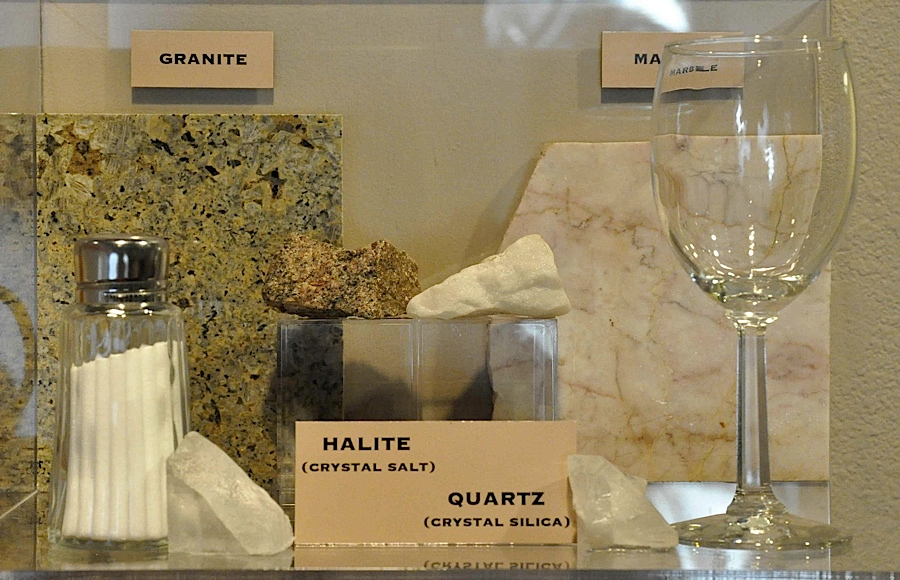
\includegraphics{shelf03}
		\centering
	\end{figure}

\pagebreak

\section{Sulfur and Flint}

	\begin{itemize}
		\item \textbf{Sulfur} is an integral part of gunpowder and matches
		\item \textbf{Flint} is a form of quartz.
	\end{itemize}
	
	\begin{figure}[h]
		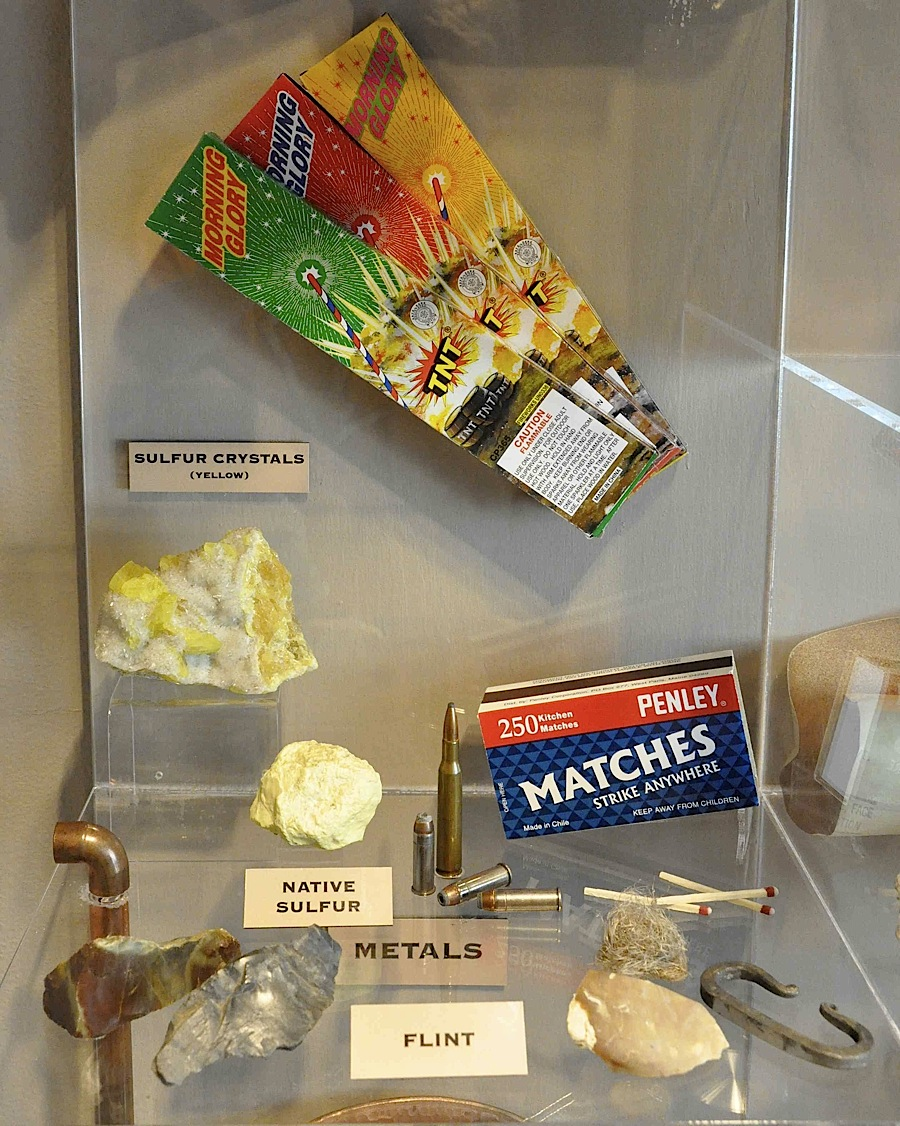
\includegraphics[height=6cm]{shelf04}
		\centering
	\end{figure}

\section{Garnet and Talc}

	\begin{itemize}
		\item \textbf{Garnet} is a gemstone used as \textbf{abrasive} for both sand blasting and sand paper.
		\item \textbf {Talc} is used in \textbf{baby powder}.
	\end{itemize}
	
	\begin{figure}[h]
		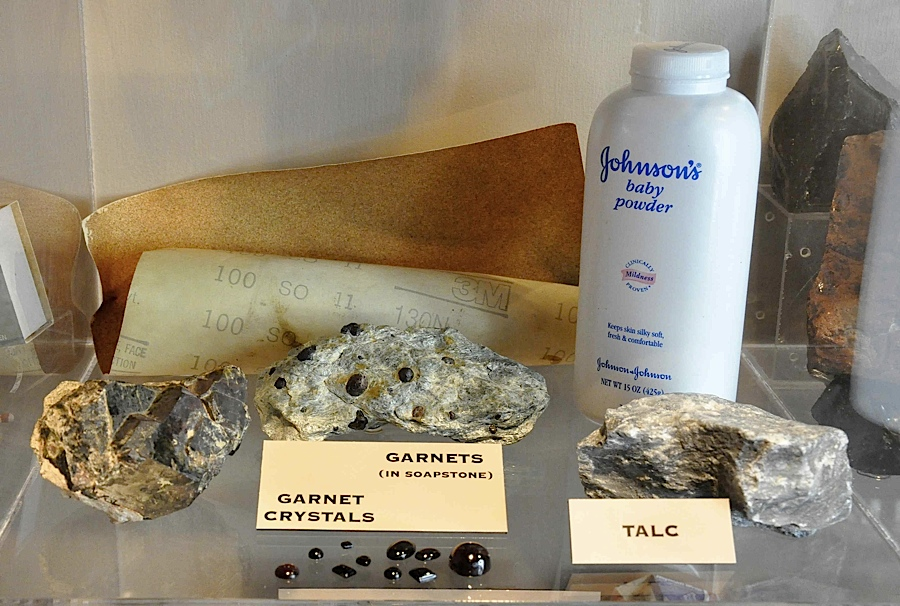
\includegraphics[height=4cm]{shelf05_0}
		\centering
	\end{figure}

	
\section{Pumice and Obsidian}

	\begin{itemize}
		\item \textbf{Obsidian} is a extremely hard rock used for \textbf{surgical scalpels}
		\item \textbf{Pumice} is used as and \textbf{abrasive}
	\end{itemize}
	
	\begin{figure}[h]
		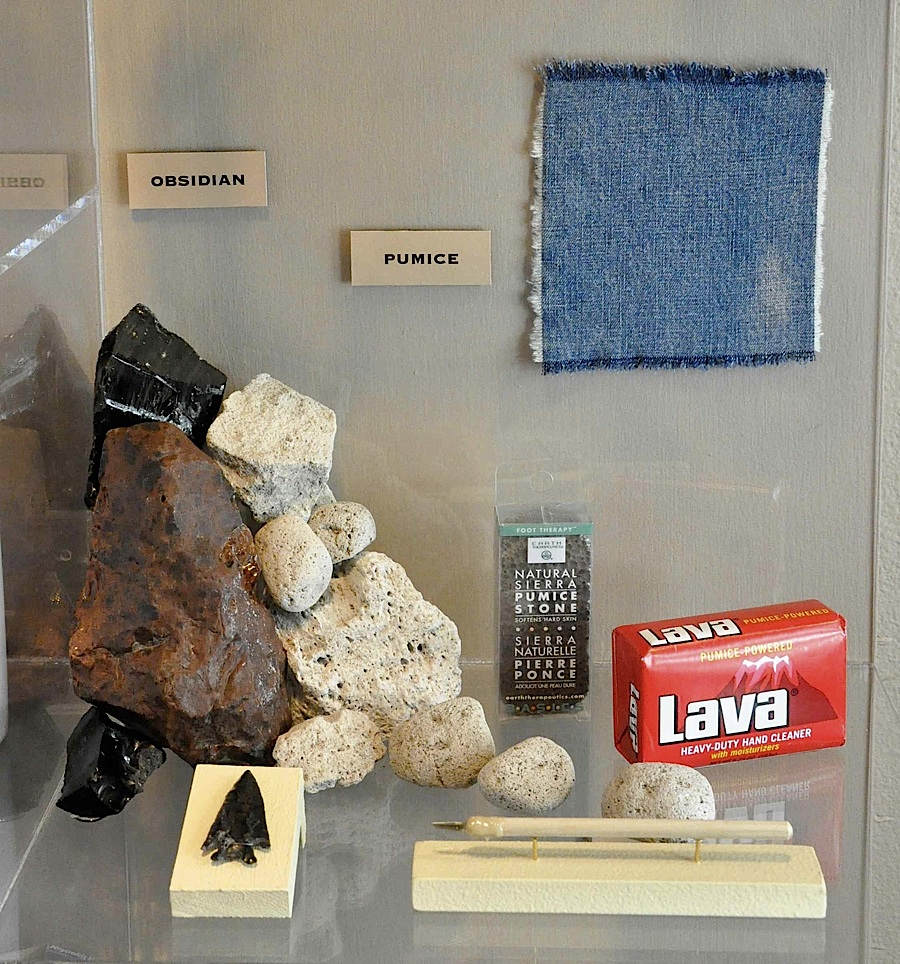
\includegraphics[height=5cm]{shelf06}
		\centering
	\end{figure}
	
\section{Copper and Zinc}

	\begin{itemize}
		\item \textbf{Copper} has low resistance to electrical charge and is abundant, so it is used for \textbf{wiring}
		\item \textbf{Zinc} is and essential element and can be taking as a supplement. It is also used for \textbf{galvanizing} to prevent coating.
	\end{itemize}
	
	\begin{figure}[h]
		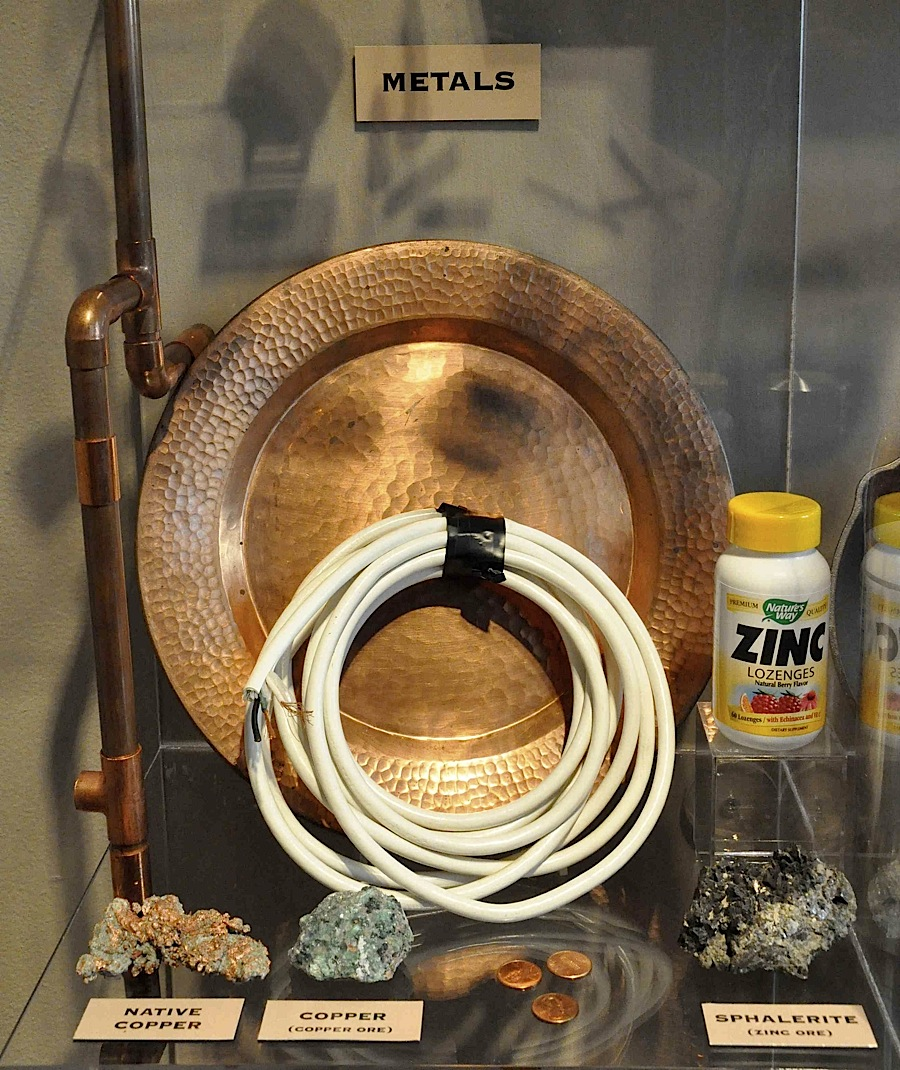
\includegraphics[height=5cm]{shelf07_0}
		\centering
	\end{figure}

\pagebreak

\section{Iron and Aluminum}

	\begin{itemize}
		\item \textbf{Iron} is commonly used in different compound with carbon and silicon.
		\item \textbf{Alumimun} was a rare and valuable metal in the 18th and 19th centuries, until it could be purified using electricity, becoming cheap and plentiful.
	\end{itemize}
	
	\begin{figure}[h]
		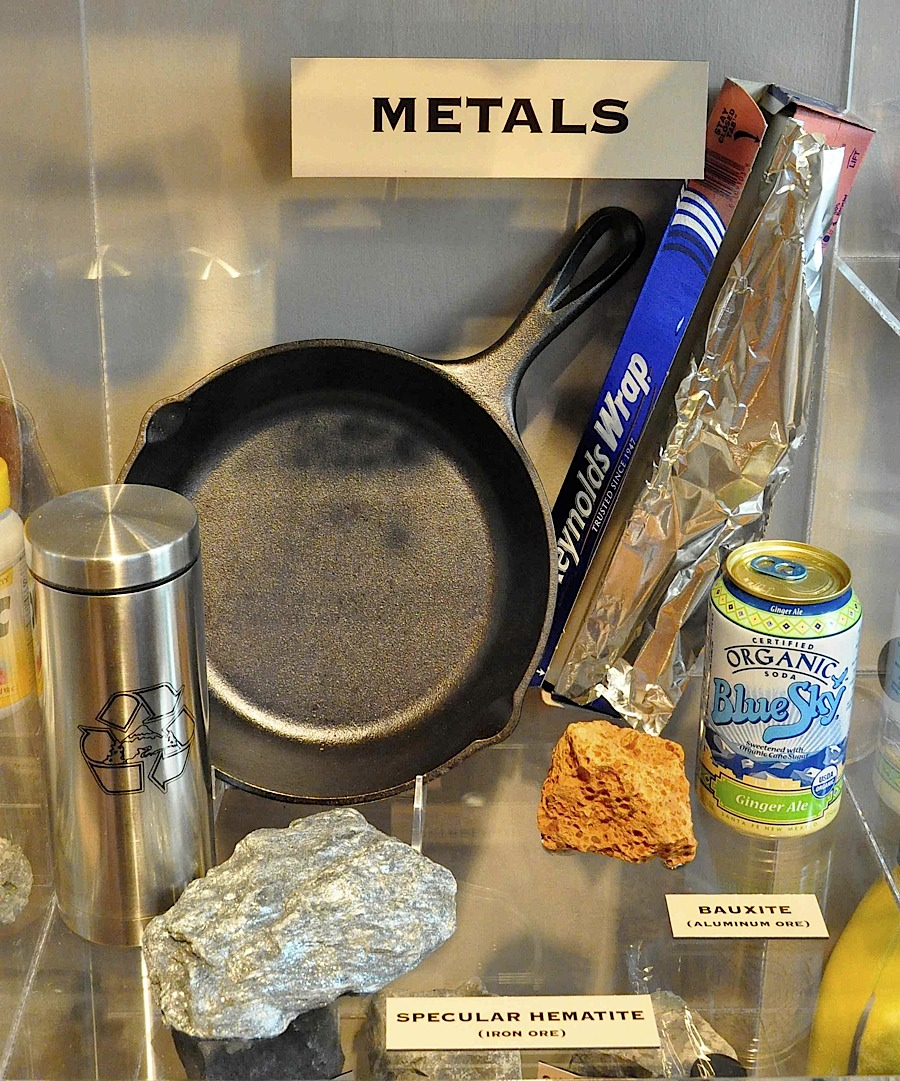
\includegraphics[height=5cm]{shelf08_0}
		\centering
	\end{figure}
	
\section{Silver and Gold}

	\textbf{Silver} and \textbf{gold} have similar chemical characteristics than copper. They are good conductors of heat and electricity, which is why they're used in high-end electronic devices.
	
	\begin{figure}[h]
		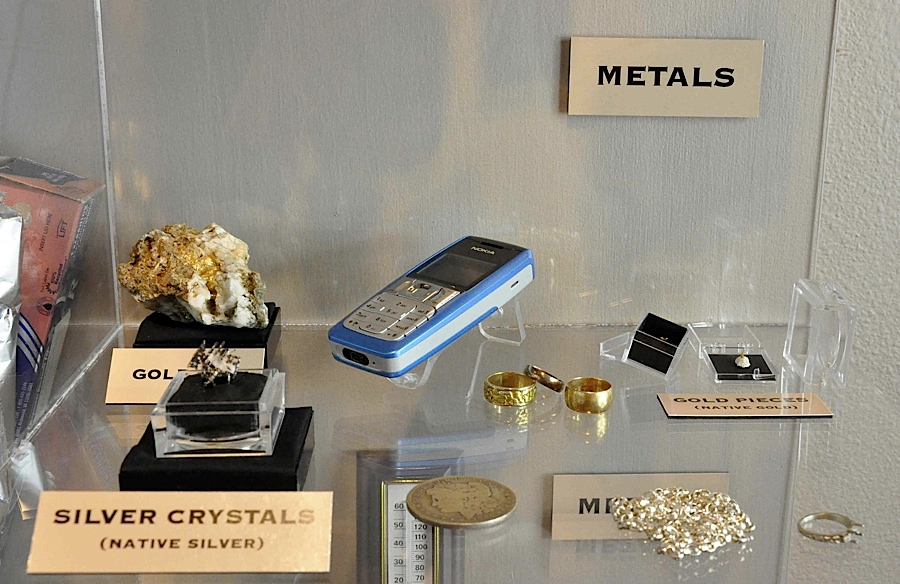
\includegraphics{shelf09}
		\centering
	\end{figure}



\section{Mercury and Lead}
	\begin{itemize}
		\item \textbf{Mercury} is the only metal that is liquid at room temperature, and that's why it has been used in thermometers. Elemental mercury is poisinous.
		\item \textbf{Lead} has been used in bullets, fishing weights, protection from X-rays. Its most common use today is in the lead-acid batteries of automobiles.  
	\end{itemize}
	
	\begin{figure}[h]
		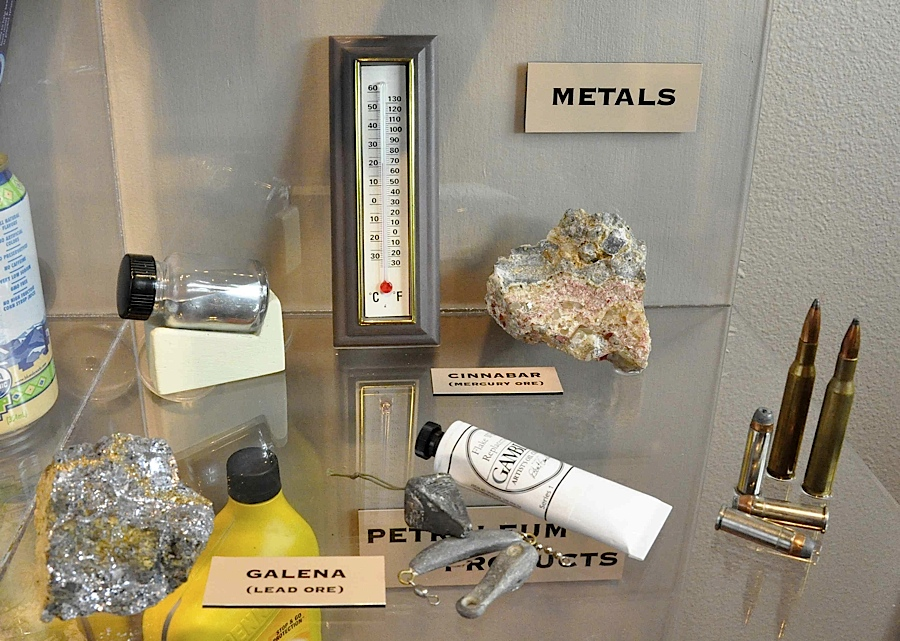
\includegraphics{shelf10}
		\centering
	\end{figure}
	
\section{Limestone, Sand and Gravel}
	To make \textbf{concrete} we mix \textbf{sand} and \textbf{gravel} with \textbf{cement}. Cement is created by heating ground \textbf{limestone} with other minerals. 
	
	\begin{figure}[h]
		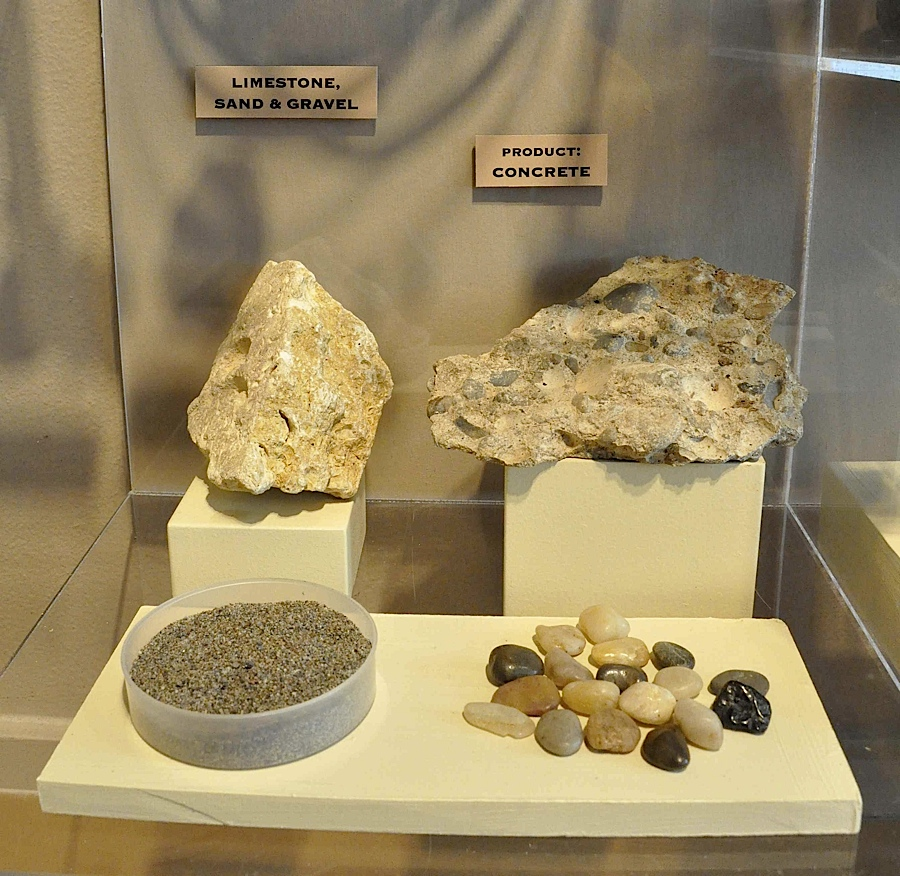
\includegraphics[height=5cm]{shelf11}
		\centering
	\end{figure}
\pagebreak

\section{Oil, Coal and Graphite}
	\begin{itemize}
		\item \textbf{Oil} contains energy from the sun trapped by organisms million of years ago. Oil is also used as machine lubricant. Rubber and plastics are made from oil.
		\item \textbf{Coal} is the remains of woody plants that died in swampy conditions.
		\item \textbf{Graphite} is elemental carbon, just lije diamond. Graphite is formed under much lower pressures and has a structure that makes slippery and easy to break
	\end{itemize}
	
	\begin{figure}[h]
		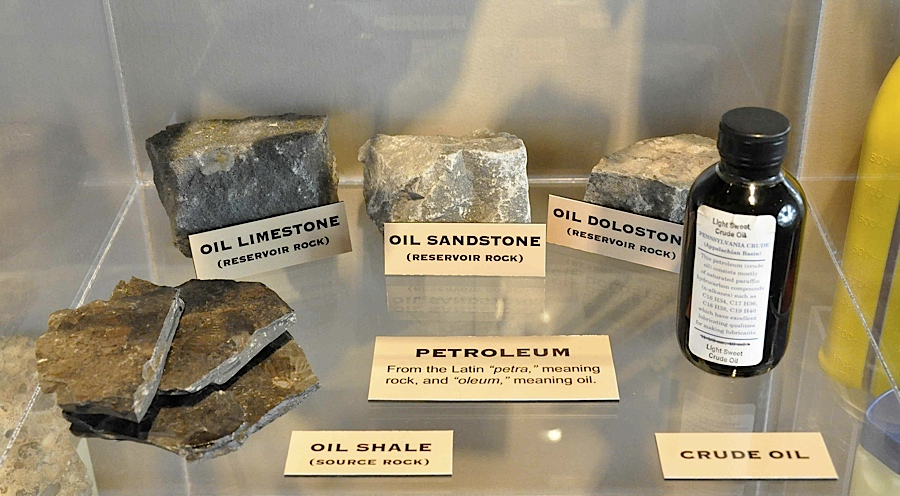
\includegraphics[height=6cm]{shelf12}
		\centering
	\end{figure}

\end{document}